
\documentclass{beamer}
\usepackage{ucs}
\usepackage[utf8x]{inputenc}
\usepackage[T1]{fontenc}

\usepackage{graphicx}
\usepackage{tipa}

\usepackage{hyperref}
\usepackage{graphics}


\begin{document}
\title{A constraint grammar for Faroese}
\author{Trond Trosterud \\ 
University of Tromsø \begin{figure}  \scalebox{0.10}[0.10]{
\includegraphics{img/LogoEngelsk}} \end{figure} 
}

\date

\frame{\titlepage} 

\frame{\frametitle{Contents}\tableofcontents} 

\section{Introduction} 

\begin{frame}
\frametitle{Background}
\begin{itemize}
\item Infrastructure from the Sámi parser project (\textit{giellatekno.uit.no})
\item The same file setup, Makefiles, etc.
\end{itemize}
\end{frame}


\begin{frame}
\frametitle{Background}
\begin{itemize}
\item Technological background
\begin{itemize}
\item Finite transducers from Xerox: \textit{twolc} for morphophonologi and \textit{lexc} for lexicon
\item CG: \textit{vislcg3}
\end{itemize}
\end{itemize}
\end{frame}

\begin{frame}
\frametitle{Background}
\begin{itemize}
\item Lexicon and grammar
\begin{itemize}
\item Føroysk órðabók, lemmalist and inflection codes electronically accessible
\item Thráinsson, Petersen, í Lon Jacobsen, Hansen: \textit{Faroese: An overview and reference grammar}
\end{itemize}
\end{itemize}
\end{frame}



\frame{\frametitle{Overview of the analyser}

\begin{itemize}
\item {Lexicon}
\item Fst transducer
\item CG disambiguator
\item CG dependency
\end{itemize}
}



\section{The morphological analyser}
\begin{frame}
\frametitle{Lexicon}

\begin{itemize}
\item The analyser uses the same inflectional codes as  \textit{Føroysk orðabók} 
\item The analyser has a dynamic compounding component (gen. sg. -> Nouns)
\end{itemize}
\end{frame}

\frame{\frametitle{Lexicon format - nouns} 
\scalebox{0.50}[0.50]{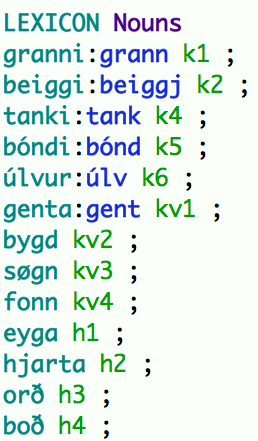
\includegraphics{img/nounlexicon.png}} \\
}


\begin{frame}
\frametitle{Morphology in three layers}
\begin{enumerate}
\item Part of speech and gender tag, morphophonological flags
\item Case and number morphology
\item Definiteness morphology
\end{enumerate}
\end{frame}



\frame{\frametitle{The name guesser}
Based upon capital first letter and non-Faroese phonotax the guesser is very reliable: 

Of the 500 most common guesses all 500 were actually names. 
}



\begin{frame}
\frametitle{Status quo for Ffst}
\begin{itemize}
\item The parser recognises 94.3 \% of the wordforms and 63.3  \% of the wordform types in running text
\item  the discrepancy indicates that Ffst handles common words better than rare ones
\item{Certain common forms are missing (some strong verbs, irregular adjective forms, comparatives (partly))}
\item{Faroese names are missing (except the most central person names}
\end{itemize}
\end{frame}


\frame{\frametitle{Lexicon format - nouns} 
\scalebox{0.33}[0.33]{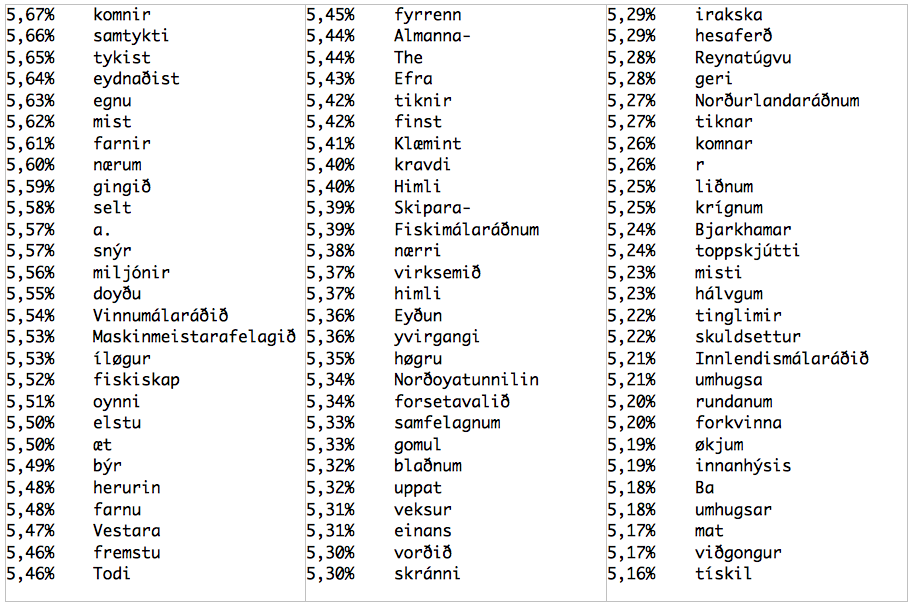
\includegraphics{img/missing.png}} \\
}


\frame{\frametitle{The missing words}
The 43093 missing words represent 5.67\% of the 2.7 mill corpus. In order to half the number of missing words, the top 2117 words of the missing list have to be added.
}

\frame{\frametitle{The Faroese disambiguator}

The disambiguator (Fdis) consists of

\begin{itemize} 
\item 120 rules for morphological disambiguation, 
\item 49 mapping rules, 
\item 46 rules for GF-disambiguation. 
\end{itemize}
}


\frame{\frametitle{Small, but relatively efficient rule set}

\begin{table}[htdp]
\caption{default}
\begin{center}
\begin{tabular}{|l|r|r|r|}
Parser & Rules & Ambiguity & Accuracy \\
\hline
North Sámi	  & 3537 & 2.42 & 1.08 \\
Norsk Bokmål  & 1964 & 2.13 & 1.17 \\
Lule Sámi	  &  832 & 2.18 & 1.21 \\
Greenlandic	  &  518 & 2.69 & 1.42 \\
Faroese		  &  294 & 2.45 & 1.24 \\
\hline
\end{tabular}
\end{center}
%\label{default}
\end{table}%

-> Fdis is work in progress 
}


\begin{frame}
\frametitle{Accuracy}

but partly it illustrates the efficiency of an innovation in vislcg3, namely set unification for tags. 

With the set unification operator \$\$ it is possible to refer to a set, so that the tag that first satisfies the set must be the same as all subsequent matches of the same set.

SET NAGD = Nom Acc Gen Dat ;

SELECT \$\$NAGD IF (0 Det)(*1C \$\$NAGD BARRIER NOT-NP);

\end{frame}


\section{The disambiguator}
\frame{\frametitle{The disambiguator}

The bulk of the rules aims at disambiguating case, number and gender within the NP. 

One clue as to determining the correct case is the choice of preposition, as it is for the human listener. 

Unfortunately, most Faroese prepositions subcategorise for more than one case. What case to choose if there is a tie is ultimately dependant upon the combination of verb and preposition. 

At the present stage, Fdis does not specify subcategorisation frames for verbs and verb + preposition combinations, this is an area for future improvement.

}


\frame{\frametitle{High-frequent ambiguous words}

When disambiguating running text, certain high-frequent words need special attention, both because they get multiple interpretations in the morphological component, and for their key role in the sentence. 

A common strategy for such words is to write specific rules just for these words. 

For Fdis, only approximately 15 such words have received special treatment until now:

\begin{description}
\item[Pronouns:] \textit{hon, vit}
\item[Subjunctions:] \textit{at, ið, men}
\end{description}


}


\frame{\frametitle{Verb homonymy}

The Faroese verbal paradigm shows much homonymy. 

Ffst specifies 3 persons in the singular (also when the conjugation in question shows homonymy), 

but only one plural form. 
}


\frame{\frametitle{Grammatical functions}

\begin{itemize}
\item Mapping of grammatical functions by
\begin{itemize}
\item morphological cues
\item word order
\end{itemize}
\item and disambiguation of grammatical functions
\begin{itemize}
\item word order
\end{itemize}
\item The grammatical function tags are directional ( @OBJ> / @<OBJ )
\item This distinction is heavily utilised in the dependency grammar.
\end{itemize}
}

\section{The dependency grammar}
\frame{\frametitle{The dependency grammar}

The dependency grammar (Fdep) consists of 49 rules. 

The dependency grammar quite reliably delimits NPs, and the governed constituents of P and V. Eventual errors here are due to errors in Fdis. 

The main obstacles for a good depencency analyses are coordination and relative clauses. Attaching appropriate constituents to the clause mother node is quite a reliable process as long as the rest of the analysis is correct. 

Unfortunately shortcomings in coordination and relative clause analysis, and especially the low coverage of the Ffst gives too many top nodes 

(2.3 alleged clausal heads per clause on average, compared to the correct 1 head/clause). 

Even with these shortcomings, the Fdep is already at this stage a good tool for research on basic dependency relations.
}

\section{Processing speed}
\frame{\frametitle{Processing speed}

the bottleneck in the system is the disambiguator. 

Even though it is much smaller than most CG grammars, it performs clearly worse than all the other parts of the pipeline.

The reason for this might be the extensive use of set unification.

\begin{table}[htdp]
\caption{Processing speed, measured on 100000 words of running text, on a 2,4 GHz laptop}
\begin{center}
\begin{tabular}{|l|l|r|}
\hline
Process & Program & Words/sec \\
\hline
Preprocessing & perl &10446 \\
Morphological lookup & fst & 42992 \\
Postprocessing & perl & 13017 \\
Disambiguation & vislcg3 & 2042 \\
Dependency & vislcg3 & 18814 \\
\hline
\end{tabular}
\end{center}
\label{time}
\end{table}%




}


\frame{\frametitle{Conclusion}

The Faroese grammatical analyser presented here is still in the making. 

It still shows that with a modest number of CG rules, one may achive results good enough for several languaguage processing tasks. 

Future improvements of the analyser will concentrate upon key parts of the Ffst, upon disambiguation of complex syntactic patterns, and upon the dependency analysis of coordination and relative clauses.

}	
\end{document}
